\documentclass[11pt,a4paper, dvipdfmx]{jsarticle}
\usepackage{amsmath,amssymb}
\usepackage{amsthm}
\usepackage{ascmac}
\usepackage{bm}
\usepackage[dvipdfmx]{graphicx}	% required for `\includegraphics' (yatex added)
\usepackage{setspace}           % required for `\doublespace'
\usepackage{tikz}
\usepackage{tikz-cd}
\usetikzlibrary{angles, positioning, shapes, arrows.meta, decorations.pathmorphing}
%\usetikzlibrary{intersections, calc, arrows, positioning, arrows.meta}
\usepackage{tcolorbox}  % 定理環境の装飾
\tcbuselibrary{skins, breakable, theorems}
\usepackage{xcolor}
\usepackage{natbib}
\usepackage{pxrubrica}
\usepackage[margin=30truemm, left=40truemm, right=40truemm]{geometry}
\usepackage{thmbox}     % required for theorem environment with side bar
%
\setlength{\parskip}{3mm} %段落間にスペースを入れる


% \pagestyle{myheadings}
% \markright{\footnotesize \sf 2022秋期「哲学者のための数学」授業資料(大塚淳) \ \ 配布禁止}


\theoremstyle{definition}
\newtheorem[S]{exercise}{練習問題}[section]
\newtheorem[S]{example}{事例}[section]
\newtheorem[S]{fact}{事実}[section]
\newtheorem[S]{attn}{注意}[section]
\newtheorem[S]{develop}{発展}[section]
\renewcommand{\theattn}{}

\newtcbtheorem[auto counter, number within=section]{rei}{事例}{
    breakable,
    coltitle=black,
    fonttitle=\bfseries,
    enhanced, colback=white, frame hidden, borderline west = {0.5pt}{5pt}{black},
%    number freestyle={\noexpand\thesection.\noexpand\arabic{\tcbcounter}}
}{rei}

\newtcbtheorem[auto counter, number within=section]{prop}{命題}{
    breakable,
    coltitle=black,
    fonttitle=\bfseries,
    enhanced, colback=white, frame hidden, borderline west = {0.5pt}{5pt}{black},
%    number freestyle={\noexpand\thesection.\noexpand\arabic{\tcbcounter}}
}{prop}

\newtcbtheorem[number within=section]{renshu}{練習問題}{
    breakable,
    coltitle=black,
    fonttitle=\bfseries,
    enhanced, colback=white, frame hidden, borderline west = {0.5pt}{5pt}{black}
}{renshu}


\newtcbtheorem[number within=section]{hatten}{発展}{
    breakable,
    coltitle=black,
    fonttitle=\bfseries,
    enhanced, colback=white, frame hidden, borderline west = {0.5pt}{5pt}{black}
}{renshu}


\newtcbtheorem[number within=section]{dfn}{定義}{
    fonttitle=\bfseries,
    enhanced, colback=white
}{dfn}


% Bold face capital letters:
\newcommand{\bfzero}{\boldsymbol{0}}
\newcommand{\bfone}{\boldsymbol{1}}
\newcommand{\bfA}{\boldsymbol{A}}
\newcommand{\bfB}{\boldsymbol{B}}
\newcommand{\bfC}{\boldsymbol{C}}
\newcommand{\bfD}{\boldsymbol{D}}
\newcommand{\bfE}{\boldsymbol{E}}
\newcommand{\bfF}{\boldsymbol{F}}
\newcommand{\bfG}{\boldsymbol{G}}
\newcommand{\bfH}{\boldsymbol{H}}
\newcommand{\bfI}{\boldsymbol{I}}
\newcommand{\bfJ}{\boldsymbol{J}}
\newcommand{\bfK}{\boldsymbol{K}}
\newcommand{\bfL}{\boldsymbol{L}}
\newcommand{\bfM}{\boldsymbol{M}}
\newcommand{\bfN}{\boldsymbol{N}}
\newcommand{\bfO}{\boldsymbol{O}}
\newcommand{\bfP}{\boldsymbol{P}}
\newcommand{\bfQ}{\boldsymbol{Q}}
\newcommand{\bfR}{\boldsymbol{R}}
\newcommand{\bfS}{\boldsymbol{S}}
\newcommand{\bfT}{\boldsymbol{T}}
\newcommand{\bfU}{\boldsymbol{U}}
\newcommand{\bfV}{\boldsymbol{V}}
\newcommand{\bfW}{\boldsymbol{W}}
\newcommand{\bfX}{\boldsymbol{X}}
\newcommand{\bfY}{\boldsymbol{Y}}
\newcommand{\bfZ}{\boldsymbol{Z}}

\newcommand{\bfa}{\boldsymbol{a}}
\newcommand{\bfb}{\boldsymbol{b}}
\newcommand{\bfc}{\boldsymbol{c}}
\newcommand{\bfd}{\boldsymbol{d}}
\newcommand{\bfe}{\boldsymbol{e}}
\newcommand{\bff}{\boldsymbol{f}}
\newcommand{\bfk}{\boldsymbol{k}}
\newcommand{\bfm}{\boldsymbol{m}}
\newcommand{\bfn}{\boldsymbol{n}}
\newcommand{\bfo}{\boldsymbol{o}}
\newcommand{\bfp}{\boldsymbol{p}}
\newcommand{\bfq}{\boldsymbol{q}}
\newcommand{\bfr}{\boldsymbol{r}}
\newcommand{\bfs}{\boldsymbol{s}}
\newcommand{\bft}{\boldsymbol{t}}
\newcommand{\bfu}{\boldsymbol{u}}
\newcommand{\bfv}{\boldsymbol{v}}
\newcommand{\bfw}{\boldsymbol{w}}
\newcommand{\bfx}{\boldsymbol{x}}
\newcommand{\bfy}{\boldsymbol{y}}
\newcommand{\bfz}{\boldsymbol{z}}



% BB (???) capital letters:
\newcommand{\bbA}{\mathbb{A}}
\newcommand{\bbB}{\mathbb{B}}
\newcommand{\bbC}{\mathbb{C}}
\newcommand{\bbD}{\mathbb{D}}
\newcommand{\bbE}{\mathbb{E}}
\newcommand{\bbF}{\mathbb{F}}
\newcommand{\bbG}{\mathbb{G}}
\newcommand{\bbI}{\mathbb{I}}
\newcommand{\bbN}{\mathbb{N}}
\newcommand{\bbP}{\mathbb{P}}
\newcommand{\bbQ}{\mathbb{Q}}
\newcommand{\bbR}{\mathbb{R}}
\newcommand{\bbU}{\mathbb{U}}
\newcommand{\bbV}{\mathbb{V}}
\newcommand{\bbX}{\mathbb{X}}
\newcommand{\bbY}{\mathbb{Y}}
\newcommand{\bbZ}{\mathbb{Z}}
\newcommand{\bbone}{{\ifmmode\mathrm{1\!l}\else\mbox{\(\mathrm{1\!l}\)}\fi}}


% Caligraphic math capital letters:
\newcommand{\mcalA}{\mathcal{A}}
\newcommand{\mcalB}{\mathcal{B}}
\newcommand{\mcalC}{\mathcal{C}}
\newcommand{\mcalD}{\mathcal{D}}
\newcommand{\mcalE}{\mathcal{E}}
\newcommand{\mcalF}{\mathcal{F}}
\newcommand{\mcalG}{\mathcal{G}}
\newcommand{\mcalH}{\mathcal{H}}
\newcommand{\mcalI}{\mathcal{I}}
\newcommand{\mcalJ}{\mathcal{J}}
\newcommand{\mcalK}{\mathcal{K}}
\newcommand{\mcalL}{\mathcal{L}}
\newcommand{\mcalM}{\mathcal{M}}
\newcommand{\mcalN}{\mathcal{N}}
\newcommand{\mcalO}{\mathcal{O}}
\newcommand{\mcalP}{\mathcal{P}}
\newcommand{\mcalQ}{\mathcal{Q}}
\newcommand{\mcalS}{\mathcal{S}}
\newcommand{\mcalT}{\mathcal{T}}
\newcommand{\mcalU}{\mathcal{U}}
\newcommand{\mcalV}{\mathcal{V}}
\newcommand{\mcalX}{\mathcal{X}}
\newcommand{\mcalY}{\mathcal{Y}}
\newcommand{\mcalZ}{\mathcal{Z}}

% Graph nodes notations:
\newcommand{\PA}{\mathit{PA}}
\newcommand{\bfPA}{\mathbf{PA}}
\newcommand{\CH}{\mathit{CH}}
\newcommand{\bfCH}{\mathbf{CH}}
\newcommand{\DS}{\mathit{DS}}
\newcommand{\bfDS}{\mathbf{DS}}
\newcommand{\ND}{\mathit{ND}}
\newcommand{\bfND}{\mathbf{ND}}
\newcommand{\AN}{\mathit{an}}
\newcommand{\bfAN}{\mathbf{an}}
\newcommand{\pa}{\mathit{pa}}
\newcommand{\bfpa}{\mathbf{pa}}
\newcommand{\ch}{\mathit{ch}}
\newcommand{\bfch}{\mathbf{ch}}
\newcommand{\ds}{\mathit{ds}}
\newcommand{\bfds}{\mathbf{ds}}
\newcommand{\nd}{\mathit{nd}}
\newcommand{\bfnd}{\mathbf{nd}}
\newcommand{\an}{\mathit{an}}
\newcommand{\bfan}{\mathbf{an}}



\DeclareMathOperator*{\argmax}{arg\,max}
\DeclareMathOperator*{\argmin}{arg\,min}
\DeclareMathOperator*{\argsup}{arg\,sup}
\DeclareMathOperator*{\arginf}{arg\,inf}
\DeclareMathOperator{\erfc}{erfc}
\DeclareMathOperator{\diag}{diag}
\DeclareMathOperator{\cum}{cum}
\DeclareMathOperator{\sgn}{sgn}
\DeclareMathOperator{\tr}{tr}
\DeclareMathOperator{\spn}{span}
\DeclareMathOperator{\adj}{adj}
\DeclareMathOperator{\E}{\mathbb{E}}
\DeclareMathOperator{\var}{Var}
\DeclareMathOperator{\cov}{Cov}
\DeclareMathOperator{\corr}{corr}
\DeclareMathOperator{\sech}{sech}
\DeclareMathOperator{\sinc}{sinc}
\DeclareMathOperator*{\lms}{l.i.m.\,}
\newcommand{\varop}[1]{\var\left[{#1}\right]}
\newcommand{\covop}[2]{\cov\left({#1},{#2}\right)}
\newcommand{\T}{^\textrm{T}}
\newcommand\indep{\protect\mathpalette{\protect\independenT}{\perp}}
\def\independenT#1#2{\mathrel{\rlap{$#1#2$}\mkern2mu{#1#2}}}

\newcommand{\bfalpha}{\boldsymbol{\alpha}}
\newcommand{\bfbeta} {\boldsymbol{\beta}}
\newcommand{\bfgamma}{\boldsymbol{\gamma}}
\newcommand{\bfeta}  {\boldsymbol{\eta}}
\newcommand{\bftheta}{\boldsymbol{\theta}}
\newcommand{\bflambda}   {\boldsymbol{\lambda}}
\newcommand{\bfmu}   {\boldsymbol{\mu}}
\newcommand{\bfnu}   {\boldsymbol{\nu}}
\newcommand{\bfxi}   {\boldsymbol{\xi}}
\newcommand{\bfpsi}  {\boldsymbol{\psi}}
\newcommand{\bfphi}   {\boldsymbol{\phi}}
\newcommand{\bfrho}   {\boldsymbol{\rho}}
\newcommand{\bfvarepsilon}{\boldsymbol{\varepsilon}}
%\newcommand{\qed}{{qed}}
%\newcommand{\eqalignno}[1]{\begin{array}{ccccccc}#1\end{array}}

\newcommand{\bfGamma}{\boldsymbol{\Gamma}}
\newcommand{\bfTheta}{\boldsymbol{\Theta}}
\newcommand{\bfLambda}   {\boldsymbol{\Lambda}}
\newcommand{\bfPsi}  {\boldsymbol{\Psi}}
\newcommand{\bfPhi}   {\boldsymbol{\Phi}}
\newcommand{\bfSigma}  {\boldsymbol{\Sigma}}
\newcommand{\bfOmega}  {\boldsymbol{\Omega}}


% DISTRIBUTIOoNS: 
\newcommand{\normal}{\mathcal{N}}
\newcommand{\binomial}{\mathcal{B}}
\newcommand{\multinomial}{\mathcal{M}}
\newcommand{\exponential}{\mathcal{E}}
\newcommand{\geometric}{\mathcal{G}}
\newcommand{\poisson}{\mbox{Poisson}}
\newcommand{\uniform}{\mbox{Uniform}}

% Logic
\newcommand{\true}{\texttt{true}}
\newcommand{\false}{\texttt{false}}


%PSTricks (commande for latent nodes)
\newcommand{\lnode}[4]{ \cnode(#1){#2}{#3}\rput(#1){\footnotesize#4} }

% KEEPING TRACK OF WORK
\newcommand{\todo}[1]
{
{\color{red}{
[TODO: #1]}}
\addcontentsline{toc}{subsection}{TO DO: #1}
}

\newcommand{\fixme}[1]{{\color{red}{#1}}}

\newenvironment{answer}[1]
{\par \color{blue}{#1}}
{}


\newcommand{\note}[2]
{
{\color{red}{
[#1: #2]}}
}




\makeatletter
% define \citepos for posesive citation (e.g. Otsuka's (2015))
\DeclareRobustCommand\citepos
  {\begingroup
   \let\NAT@nmfmt\NAT@posfmt% ...except with a different name format
   \NAT@swafalse\let\NAT@ctype\z@\NAT@partrue
   \@ifstar{\NAT@fulltrue\NAT@citetp}{\NAT@fullfalse\NAT@citetp}}

\let\NAT@orig@nmfmt\NAT@nmfmt
\def\NAT@posfmt#1{\NAT@orig@nmfmt{#1's}}
\makeatother




% Code for drawing color circle used in topology (pathconnectedness)
\usepackage{xparse}
\ExplSyntaxOn

\keys_define:nn { colour_transition_circle } {
    inner   .fp_set:N   = \l__inner_radius,
    inner   .initial:n  = {2},
    outer   .fp_set:N   = \l__outer_radius,
    outer   .initial:n  = {3},
    angle   .fp_set:N   = \l__start_angle,
    angle   .initial:n  = {0}
}

\NewDocumentCommand \ColourTransitionCircle { O{} m } {
\group_begin:
    \keys_set:nn { colour_transition_circle } {#1}
    \clist_clear:N \l_tmpa_clist
    \clist_map_inline:nn {#2} {
        \clist_put_right:Nn \l_tmpa_clist {##1}
        %\clist_put_right:Nn \l_tmpa_clist {##1}
    }
    \exp_args:Nx \col_trans_circ:n \l_tmpa_clist
\group_end:
}

\cs_new_protected:Npn \col_trans_circ:n #1 {
    \int_step_inline:nnnn {1} {1} {\clist_count:n {#1} - 1} {
        \path[top~color=\clist_item:nn {#1} {##1}, bottom~color=\clist_item:nn {#1} {##1+1}, shading~angle={270-(180-360/\clist_count:n {#1})/2+(##1-1)*360/\clist_count:n {#1}+\fp_use:N \l__start_angle}] ({\fp_use:N \l__inner_radius*cos((##1-1)*360/\clist_count:n {#1}+\fp_use:N \l__start_angle)},{\fp_use:N \l__inner_radius*sin((##1-1)*360/\clist_count:n {#1}+\fp_use:N \l__start_angle)}) arc[radius = \fp_use:N \l__inner_radius, start~angle={(##1-1)*360/\clist_count:n {#1}+\fp_use:N \l__start_angle}, delta~angle=360/\clist_count:n {#1}] -- ({\fp_use:N \l__outer_radius*cos(##1*360/\clist_count:n {#1}+\fp_use:N \l__start_angle)},{\fp_use:N \l__outer_radius*sin(##1*360/\clist_count:n {#1}+\fp_use:N \l__start_angle)}) arc[radius = \fp_use:N \l__outer_radius, start~angle={##1*360/\clist_count:n {#1}+\fp_use:N \l__start_angle}, delta~angle=-360/\clist_count:n {#1}] -- cycle;
    }
    \path[top~color=\clist_item:nn {#1} {\clist_count:n {#1}}, bottom~color=\clist_item:nn {#1} {1}, shading~angle={180-180/\clist_count:n {#1}+\fp_use:N \l__start_angle}]({\fp_use:N \l__inner_radius*cos((\clist_count:n {#1}-1)*360/\clist_count:n {#1}+\fp_use:N \l__start_angle)},{\fp_use:N \l__inner_radius*sin((\clist_count:n {#1}-1)*360/\clist_count:n {#1}+\fp_use:N \l__start_angle)}) arc[radius = \fp_use:N \l__inner_radius, start~angle={(\clist_count:n {#1}-1)*360/\clist_count:n {#1}+\fp_use:N \l__start_angle}, delta~angle=360/\clist_count:n {#1}] -- ({\fp_use:N \l__outer_radius*cos(\clist_count:n {#1}*360/\clist_count:n {#1}+\fp_use:N \l__start_angle)},{\fp_use:N \l__outer_radius*sin(\clist_count:n {#1}*360/\clist_count:n {#1}+\fp_use:N \l__start_angle)}) arc[radius = \fp_use:N \l__outer_radius, start~angle={\clist_count:n {#1}*360/\clist_count:n {#1}+\fp_use:N \l__start_angle}, delta~angle=-360/\clist_count:n {#1}] -- cycle;
}

\ExplSyntaxOff
\usepackage{xcolor}

\begin{document}


\title{5. 位相}
\author{2023秋期「哲学者のための数学」授業資料(大塚淳)}
\date{ver. \today}
\maketitle

\section{位相とは何か・なぜそれを学ぶのか}

本章の主題は位相(topology)である.
大雑把にいうと,位相とは空間についての学問であり,近さや距離といったものを扱うための道具立てを与える.
我々が見てきた集合は,いわばそれぞれが独立した,つぶつぶの要素の集まりであって,その間の近さや距離みたいなものは考えられていなかった.
確かに空間や円・線などの幾何学的図形は点の集まりすなわち集合ではあるのだが,単なる集合には我々が「空間」に期待する様々な性質,例えば点と点の間の距離や近さといったものが備わっていない.
位相は,こうした幾何学的な性質を集合に与える.
その意味で,位相空間(位相が備わった集合)は,最もプリミティブで抽象的な意味での「空間」の概念だということができる\footnote{プリミティブ,というのは,例えば物理学などでおなじみの空間概念は,位相以外の条件をさらに必要とするからだ.具体的には,それらは多様体(manifold)といわれる,のであるが,本講では扱わない.}.

このような次第で,位相は物理学等において非常に重要な役割を持っている一方,哲学においては,それほど重視されてこなかった.
しかしながら,空間や近さという概念は,哲学においても頻出の重要概念である.
多くの場合,そうした議論では暗にユークリッド空間がイメージされることが多いが,ユークリッド空間というのは実は非常に特殊で「リッチ」な空間概念なので,そのイメージに引きづられると物事の理解を歪めてしまうかもしれない.
それを防ぐためにも,位相一般についての知識を持っていることは望ましい.

位相を考えるには,二つのアプローチがある.
一つは,集合上に距離を導入して,距離空間(距離が定められた集合)の上で位相的性質を定めていく方法.
もう一つは,集合上のそれぞれの点の間の類似性を示すグルーピング(これを「開集合」と呼ぶ)を与えて,そこから距離を導く方法.
%これらはトンネルを右から掘るか左から掘るかの違いのようなもので,最終的には同じことである.
前者は直感的でイメージしやすいため,数学の教科書でも前者から入るものが多い.
しかし本講では,抽象的ではあるがより哲学的な含意が見えやすい後者のアプローチをとり,位相構造を開集合の族として与えることにする.

% 類似性を表す基準としての位相
% 連続性
% 空間・幾何学の基礎(代数に対し)
% 空間というとユークリッドだが,もっとプリミティブな空間のアイデア

\section{位相空間}

前述の通り,位相空間のアプローチでは,集合上に「似た者同士」を示すグルーピングを与えることから始まる.
これは,集合$T$の部分集合を「似た者グループ」として指定していくことにほかならない.
このような「似た者グループ」としての部分集合を,\emph{開集合}(open set)という.
位相空間とは,こうした開集合の族$\mcalO$が定義された集合である.
しかし開集合の族は,一定のルールに従って構成されなければならない.
このルールが位相空間を定める公理となる.
さっそく定義を見てみよう.

\begin{dfn}{位相空間}
集合$T$の部分集合の族$\mcalO$が以下の条件を満たすとき,$\mcalO$は$T$の\emph{位相}であるといい,$T$を(位相$\mcalO$を持つ)\emph{位相空間}という.また$\mcalO$の要素である部分集合$O \subset T, O \in \mcalO$を開集合という.
\begin{enumerate}
 \item $\emptyset, T \in \mcalO$.
 \item $O_1, O_2 \in \mcalO$ならば$O_1 \cap O_2 \in \mcalO$.
 \item 任意の数(無限であっても良い)の$O_i \in \mcalO, i \in I$に対し,$\bigcup_{i \in I} O_i \in \mcalO$.
\end{enumerate}
\end{dfn}

それぞれ説明していこう.
まず条件1によれば,空集合$\emptyset$と集合全体$T$はそれぞれ開集合である.
条件2により,二つの開集合があったとき,その共通部分も開集合になっている.
これを繰り返すと,有限個の開集合の共通部分は開集合である,ということも帰結する.
条件3は,複数の開集合があったとき,その合併も開集合になる.
ただ条件2と違い,合併される開集合は無限個であっても構わない.
条件2,3を言い換えると,位相は有限個の交わりと無限個の和に対して閉じている,ということになる.

そもそもなんでこんなルール(公理)を持った集合系として位相を定義しなければならないのか?と思った人もいるかも知れないが,そこはこのように定義すると「色々上手くいく」のだと思ってとりあえずは飲み込んでいただきたい.
ただ冷静に見ると,この定義は3節で見た束に似ている.
束は全ての2元につき,結びと交わりが存在するのだった.
そして実際,$\cup,\cap$を部分集合間の結び・交わりとみなすと,公理2と3は位相空間を構成する開集合族$\mcalO$が束になっていること,そして公理1はこの束が最大元$T$と最小元$\emptyset$を持つことを保証している.
(では問題はなぜ共通部分と合併で有限/無限の微妙な違いを設けるか,ということだが,これは開集合/閉集合というものに期待される性質に関係している.定義から明らかなように,これは無限性に関係している,が,本授業ではそこまで扱えない.)

とにかく,開集合系が束をなすということから,ある有限部分集合系$\mcalO$が与えられた時,それが位相を定めるかということをチェックするためには,すべてのノードのペアについて,その合併と共通部分が結び・交わりとして$\mcalO$に含まれているかどうかを見れば良い.
例えば$T:=\{a, b, c\}$とし,開集合として$\mcalO_1 := \{ \emptyset, \{a \}, \{b\} \{a,b\}, \{a,b,c\} \}$をとってみよう.
この束構造は以下左のようになり,すべての結び・交わりが$\mcalO$に含まれているのでこれは位相を与える.
一方,$\mcalO_2 := \{ \emptyset, \{a \}, \{a,b\}, \{b,c\}, \{a,b,c\} \}$はそうではない.
これを開集合系にするためには,右図のように$\{b\} =  \{a,b\} \cap \{b,c\}$を含める必要がある.
\begin{figure}[h]
    \centering
    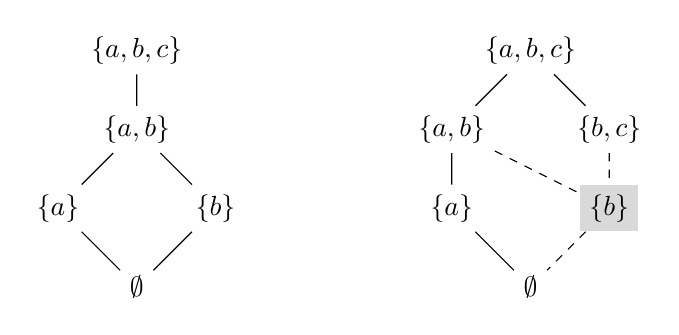
\begin{tikzpicture}
     \begin{scope}
      \node (abc)  at (1,3) {$  \{a, b, c\}$};
      \node (ab)  at (1,2) {$ \{a, b\} $};
      \node (a)  at (0,1) {$\{ a \}$};
      \node (b)  at (2,1) {$\{ b \}$};
      \node (0)  at (1,0) {$\emptyset$};
      \draw(abc)--(ab)--(a)--(0)--(b)--(ab);
     \end{scope}
     \begin{scope}[xshift=5cm]
      \node (abc)  at (1,3) {$ \{a, b, c\}$};
      \node (ab)  at (0,2) {$ \{a, b\} $};
      \node (bc)  at (2,2) {$ \{b, c\} $};
      \node (a)  at (0,1) {$\{ a \}$};
      \node[fill=gray!30] (b)  at (2,1) {$\{ b \}$};
      \node (0)  at (1,0) {$\emptyset$};
      \draw (bc)--(abc)--(ab)--(a)--(0);
      \draw[dashed] (bc)--(b)--(0);
      \draw[dashed] (ab)--(b);
     \end{scope}
    \end{tikzpicture}
    \caption{$T = \{a, b, c\}$としたときの開集合系の例$\mcalO_1$(左),$\mcalO_2$(右).}
    \label{fig:3bool} 
\end{figure}


\begin{exercise}
\label{topologyex}
同様に$T:=\{a, b, c\}$としたとき
\begin{enumerate}
\item $\mcalO_3 := \{ \emptyset, \{a \}, \{b\} \{a,b\}, \{a, c\}, \{a,b,c\} \}$
\item $\mcalO_4 := \{ \emptyset, \{b\}, \{a,b\}, \{a, c\}, \{a,b,c\} \}$
\end{enumerate}
がそれぞれ$T$の位相となっているかどうか考えよ.またなっていない場合,最低限何を足したら位相となるかを答えよ.
\end{exercise}

位相空間はもととなる集合とその上の位相のペアとして定義される.
上の事例では同じ集合$T$を用いて異なる位相$(T, \mcalO_i)$が定義されることを見た.
一般に位相空間は,このように(集合, 位相)のペアとして指定する.
しかしいちいち位相を明示せずに,「$T$を位相空間とする」というようにいうこともある.
このような表現に出くわしたら,「集合$T$の上に,何か適当な位相$\mcalO$が乗っているんだな」と補って読んでほしい.


\begin{example}
位相空間の定義はいささか抽象的すぎるので,例で考えてみる.
ここで$T$を地球上に存在する個物の集合とすると,それらに共通する\emph{性質}(property)を抜き出すことで個物を「似た者グループ」に分類することができるだろう.
例えば「赤い」という性質グループには,あなたの近所のポストや昨日食べたトマトが属する.
一方,「鉄製」というグループには,ポストは含まれるがトマトは入っていない.
このように様々な性質は異なった仕方で個物をグルーピングする.
こうして種々の性質(厳密にいうとその外延extension)は,個物の集合$T$の部分集合である.
この部分集合としての性質が$T$に位相を定めるかどうかを見るためには,上述の3つの公理が満たされるかどうかをチェックしなければならない.
\begin{enumerate}
 \item まず「無」と「存在」という性質は,それぞれ$\emptyset$と$T$自体に対応する.
 \item 二つの性質があれば,両者に共通する性質も存在する.
 \item 複数の性質があれば,「そのうちどれか一つを性質をもつ」という性質が存在する.
\end{enumerate}
これらの公理が,我々の持っている性質観と一致するか,考えてみよう.
\end{example}


位相空間に出くわしたら,それがちゃんと公理を満たしているかどうかを確認しよう.
特に,開集合族の(無限)和および(有限)共通部分がしっかりと位相に含まれているかどうかが重要である.
例えば上で,同じ性質を共有する事物を「似た者」としてグルーピングしたが,これが位相を構成するためには,複数の似た者グループ/開集合の和や共通部分もまたグループ/開集合となっているのでなければならない.
逆に,ある部分集合族が与えられたら,これらの部分集合の和や共通部分をすべて付け加えることで,位相を構成できる.
この作業を,「無限和と有限共通部分をとる」と表現することがある.

\begin{exercise}
 $T = \{$ アメリカ(A), 中国(C), 日本(J), メキシコ(M), イギリス(U) $\}$とする.
これらを何らかの基準で「似た者」とするグルーピングを考え,位相空間を構成せよ.当然この問題には答えはないが,それぞれのグループに説明があると望ましい.
\end{exercise}


\begin{example}
\label{ex:real}
数学でよく使われる位相空間の例を一つ.
実数直線$\bbR$上の\emph{開区間}(open interval)を,以下によって定める
\[
  (a, b) := \{ x \in \bbR| a < x < b \}
\]
ただし$a, b \in \bbR \cup \{-\infty, \infty\}$.
こうして得られるすべての開区間と,任意の開区間の無限和および有限共通部分をとってできる区間のすべてを開集合とすると,これは$\bbR$上の位相を定める.例えば
\begin{itemize}
 \item $(\pi,7)$
 \item $\bbR = (-\infty, \infty)$
 \item $(-\infty, 0) \cup (\sqrt{2}, \pi)$ 
\end{itemize}
などは$\bbR$上の開集合である.
\end{example}


\begin{example}
\label{possibleworlds}
いま$W$を可能世界の集合とし,$A$を命題の集合としよう.
それぞれの命題$a \in A$について,その命題が成り立っている可能世界を集めたものを$W_a \subset W$と表し,「$a$世界($a$-worlds)」と呼ぶ.
つまり$W_a := \{ w \in W | a \text{ is true in } w \}$である.
このとき,部分集合族$\{ W_a \}_{a \in A}$が位相を構成する条件を定義2.1に照らして考えてみよう.
まず,条件1より,空集合と全体集合がなければならないが,$W_{\bot} = \emptyset, W_{\top}=W$より,矛盾$\bot$とトートロジー$\top$が$A$に含まれていなければならない.
次に,
\begin{align*}
W_a \cap W_b &=  \{ w \in W | a \text{ is true in } w \} \cap \{ w \in W | b \text{ is true in } w \} \\
&= \{ w \in W | a \wedge b \text{ is true in } w \} \\
&= W_{a \wedge b}
\end{align*}
より,条件2を満たすためには$A$は有限個の$\wedge$について閉じている必要がある.
また同様に$A$が無限個の$\vee$についても閉じていれば,条件3が満たされ,可能世界の集合が位相を持つことになる.
この位相における開集合は各$a$世界であって,それは「命題$a$が成立している」という限りで「似ている」可能世界のグループを形成している.
\end{example}


\section{閉集合}
$O$が$T$の開集合のとき,その補集合(つまり$T$から$O$を除いた部分)を\emph{閉集合}(closed set)という.
閉集合を$F$,それを集めた閉集合族を$\mcalF$と書くと,
\[
 F \in \mcalF \iff F^c \in \mcalO
\]
(ただし$F^c := T \setminus F$と定めたことを思い出そう).
つまりある部分集合$F$が閉集合であるのはその補集合$F^c$が開集合であるとき,そのときのみである.

$\mcalO$が$T$の位相となっているとき,閉集合族$\mcalF$に対して以下がなりたつ.
\begin{dfn}{閉集合系による位相の定義}{closed_topology}
  \begin{enumerate}
    \item $\emptyset, T \in \mcalF$.
    \item $F_1, F_2 \in \mcalF$ならば$F_1 \cup F_2 \in \mcalF$.
    \item 任意の数(無限であっても良い)の$F_i \in \mcalF, i \in I$に対し,$\bigcap_{i \in I} F_i \in \mcalF$.
  \end{enumerate}
\end{dfn}

2と3はちょうど位相空間の定義における開集合族の規定2,3の共通部分と合併をそれぞれ入れ替えたものであることに注意.
つまり閉集合族は開集合族とは逆に,有限個の和と無限個の交わりに対して閉じている.
逆に,閉集合族がこの3つの条件を満たす時,対応する開集合族は位相の定義を満たす.
なので開集合ではなく,こちらを位相空間の定義として使っても良い.

事例\ref{ex:real}で,開集合の事例として$<$で囲まれた実数直線上の開区間を見た.
逆に,$a, b \in \bbR \cup \{-\infty, \infty\}$によって$\leq$で囲まれた閉区間(closed interval)
\[
  [a, b] := \{ x \in \bbR| a \leq x \leq b \}
\]
は閉集合の代表的事例である.
一般に開区間は丸括弧$(,)$,閉区間は角括弧$[,]$で表される.
この事例から示唆されるように,閉集合は「境界」がそのうちに含まれるのに対し,開集合はそうではない,という特徴がある(あるいは,開集合の周りの境界を含めたものが,閉集合であるともいえる).
この一見些細に見える違いが,実は非常に重要であり,そこからこの2つの概念の重要性が出てくるのであるが,本講義ではこれ以上立ち入らない.

ただ一つだけ心に留めておいてほしいのは,開集合と閉集合は,二者択一の関係ではないということだ.
例えば,片方が開でもう片方が閉であるような区間$(a, b] := \{ x \in \bbR| a < x \leq b \}$は開集合でも閉集合でもない.
また,ある部分集合$B \subset T$が閉集合であることは,必ずしもそれが開集合であることを妨げない.
実際,$\emptyset, T$は定義より開集合でありまた閉集合でもあるし,これ以外にも同時に開かつ閉であるような部分集合(\emph{clopen}と呼ばれる)がありえる.


\begin{example}
 集合$T$に対して,その位相を冪集合$\mcalP(T)$で定める,つまり$\mcalO = \mcalP(T)$と定めることができる.
 このとき,任意の部分集合$X \subset T$について,$X \in \mcalP(T)$かつ$X^c \in \mcalP(T)$であるので,$X$は開かつ閉(clopen)である.
\end{example}

\begin{example}
 事例\ref{possibleworlds}で見た可能世界の位相において,任意の命題$a \in A$について$W_a \in \mcalO$としたとき,それぞれの$a$世界$W_a$はclopenだろうか.
\end{example}


\section{さまざまな位相}
上で見てきたように,同じ集合$T$に対して,異なる位相を入れることができる.
これは上のイメージでは,「何を似たものとするか」というグルーピングの仕方は一通りではなく,様々な仕方が考えられるということだ.

まず極端なケースとして,空集合と全体集合のみを開集合とする位相空間$\mcalO = \{\emptyset, T\}$が考えられる.
これを\emph{密着位相}(coarsest topology)という.
密着位相は何も含まれないグループか,すべてを含むグループしか持たない.
だからここではすべての要素$x \in T$が一蓮托生に密着してしまっており,その中の一部だけを「似た者グループ」として取り出すことができない.

逆の極端ケースは,すべての部分集合を開集合とする位相空間$\mcalO = \mcalP(T)$である.
これを\emph{離散位相}(discrete topology)という.
ここでは,任意の部分集合が「似た者」グループを作る.
とりわけ,すべての要素$x \in T$は,それ自身が開集合$\{x\}$になっている.
なのですべての要素がより分けられてしまっていて,バラバラ(離散)になっている.

これを両端として,他にも様々な位相が考えられる.
ある位相$\mcalO_1$の開集合がすべて,別の位相$\mcalO_2$に含まれるとき,つまり$\mcalO_1 \subset \mcalO_2$のとき,$\mcalO_2$は$\mcalO_1$より\emph{細かい}(finer),$\mcalO_1$は$\mcalO_2$より\emph{粗い}(coarser)という.
$\mcalO_2$のほうが要素をより細かくグルーピングしている,というイメージだ.
この意味でいうと,密着位相は最も粗く,離散位相は最も細かい位相空間ということになる.
位相空間のモデリングでは,密着位相や離散位相はあまりおもしろくなく,対象に合わせた「ちょうどいい」細かさの位相を入れることがキモとなってくる.

\begin{exercise}
事例\ref{topologyex}でとりあげた集合 $T:=\{a, b, c\}$上の位相$\mcalO := \{ \emptyset, \{a \}, \{b\} \{a,b\}, \{a,b,c\} \}$について,(1) $\mcalO$より粗い位相,および(2)より細かい位相,をすべてあげよ.
\end{exercise}


\begin{exercise}
$T':=\{a, b, c, d\}$とする.
\begin{enumerate}
 \item 密着位相でも離散位相でもないような$T'$上の位相$\mcalO$を一つ例示せよ(ただし問2も参照せよ).
 \item 1よりも粗い位相/細かい位相をそれぞれ一つづつ例示せよ.ただし密着位相と離散位相は除く.
\end{enumerate}
\end{exercise}


\begin{develop}
事例\ref{possibleworlds}で見たように,命題の集合$A$は可能世界に位相を定める.
いま,$A \subset A'$としたとき,それぞれの命題集合によって定められる可能世界の位相$\mcalO, \mcalO'$はどんな関係にあるだろうか.特に,$\mcalO'$は$\mcalO$より細かいだろうか.
\end{develop}


% \begin{exercise}
% 有限集合$T$上の位相間の「より細かい」という関係は,どんな構造をなすだろうか.
% \end{exercise}



% 近傍?
% 内部・外部・閉包・境界

\section{連続写像}
次に,ある位相空間$X$から別の位相空間$Y$への写像を考えたい.
位相空間とは集合の上に位相である開集合族が乗っているだけなので,その集合上の写像$f:X \to Y$を位相空間$X$から$Y$への写像だと読み替えることができる.
ただしそうした写像は位相とはお構いなしに定義できるので,必ずしもそれらが$X$と$Y$の開集合を対応付けているとは限らない.
つまり,$X$の開集合$O_X$を$f$で送った像$f(O_X)$が$Y$の開集合である保証も,$Y$の開集合$O_Y$の逆像$f^{-1}(O_Y)$が$X$の開集合である保証もない.
前者の条件を満たす写像を特別に\emph{開写像}(open map),後者を満たす写像を\emph{連続写像}(continuous map)という.

\begin{dfn}{開写像と連続写像}{continous}
  $(X, \mcalO_X), (Y, \mcalO_Y)$をそれぞれ位相空間とし,$f:X \to Y$を写像とする.
  \begin{enumerate}
    \item $X$の任意の開集合$O_X \in \mcalO_X$に対し,$f$によるその像が$Y$の開集合である,つまり$f(O_X) \in \mcalO_Y$のとき,$f$を\emph{開写像}という.
    \item $Y$の任意の開集合$O_Y \in \mcalO_Y$に対し,$f$によるその逆像が$X$の開集合である,つまり$f^{-1}(O_Y) \in \mcalO_X$のとき,$f$を\emph{連続写像}という.
  \end{enumerate}  
\end{dfn}
  

開集合は「似た者同士」のグルーピングを与える,という本講のイメージに従えば,開写像は$X$でのグループが$Y$でもグループとして成立しているという意味で保存的な写像である.
一方,連続写像は$X$においてグループになっていないものは$Y$でグループにはならない,つまり写像$f$が$X$になかったグループを新たに作り出さない,という意味で保守的であるといえる.
この両者のうち,特に後者の連続写像は重要であり,位相空間における基本的な写像となっている.
そのため,以下でも連続写像に焦点をおいて考えてみよう.

\begin{example}
アナロジーとは,あるドメインから別のドメインへの,グルーピングを保存する写像として考えることができる.
例えば陸の動物の集合$X = \{lion, elephant, armadillo,...\}$から海の動物の集合$Y = \{shark, whale, turtle,...\}$への以下のような写像を考えよう:
\[
 f (lion) = shark, f(elephant)=whale, f(armadillo) = turtle,...
\]
一方$X, Y$には,各動物のグルーピング(捕食者,大きい等々)として開集合が定義されていると考える.
このとき,$Y$が$X$の良いアナロジーとなっているためには,$X$にもともと含まれないようなグルーピングが$Y$にあってしまうと都合が悪いだろう.
これは$f$が連続である,という要件にほかならない.
\end{example}

写像はその定義域の位相が細かいほど,また値域の位相が粗いほど,連続になりやすくなる.
比喩的に言い換えれば,位相が細かいところから粗いところに流れる写像ほど,連続になりやすくなる.
極端な例としては,離散位相からの写像は値域に関わらずすべて連続であり,また密着位相への写像は定義域に関わらずすべて連続である(理由を考えてみよ).
このことを,$X$から$X$への恒等写像$i:X \to X$で考えてみよう.
これはすべての$x \in X$に対して$i(x) = x$となるような,「何もしない」写像である.
$X$上の異なる位相$\mcalO, \mcalO'$を考えると,$i$は位相空間$(X, \mcalO)$から$(X, \mcalO')$の写像だと考えることができる.
このとき
\[
 i \text{ が連続 } \iff \mcalO' \subset \mcalO
\]
が成り立つ.
というのも,$i$が連続であるとは,$\mcalO'$に含まれる任意の開集合$O'$について,$i^{-1}(O')=O'$自身が$\mcalO$に含まれる,ということにほかならないからだ.
つまり同一の集合上の位相空間を考えたとき,恒等写像の連続性は位相の細かさ/粗さに正確に対応している.


% 概念体系を別の概念体系に移す
% 連続写像の条件は?

「連続」というと,高校数学で習った実数関数の連続性を思い浮かべる人もいるかもしれない.
実のところその連続性は,ここで見た位相的な連続性にほかならない.
実数の集合$X$から$Y$への関数を考える.
例\ref{ex:real}で見たように,実数上の位相は,開区間$(a,b)$とその無限和・有限共通部分からなっている.
$X$から$Y$への関数$f:X \to Y$が連続であるとは,$Y$の開区間$(a,b)$の逆像$f^{-1}(a,b)$が,$X$で開区間(ないしその無限和か有限共通部分)になっているということである.
例えば$f(x) = x^3-2x$では,$y$軸上の任意の開区間で曲線を$x$軸に投影すると,その影は開区間の和になっている.よってこの関数は連続である(図\ref{fig:realcontinuous}左).

\begin{figure}[h]
  \begin{minipage}[b]{0.45\linewidth}
    \centering
    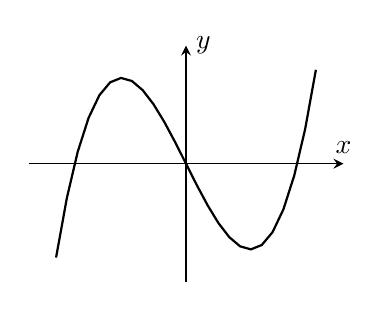
\begin{tikzpicture}[scale=1]
     \draw[->,>=stealth,semithick](-2,0)--(2,0)node[above]{$x$};%x軸
     \draw[->,>=stealth,semithick](0,-1.5)--(0,1.5)node[right]{$y$};%y軸
     \draw[thick,domain=-1.65:1.65] plot(\x,{pow(\x,3)-2*\x});
    \end{tikzpicture} 
  \end{minipage}
  \begin{minipage}[b]{0.45\linewidth}
   \begin{tikzpicture}[scale=1]
    \draw[->,>=stealth,semithick](-1,0)--(3,0)node[above]{$x$};%x軸
    \draw[->,>=stealth,semithick](0,-1.5)--(0,1.5)node[right]{$y$};%y軸
    \draw[thick,domain=-0.5:1] plot(\x,-1);
    \draw[thick,domain=1.06:2.5] plot(\x,1);
    \draw(1,1) circle [thick, radius=2pt];
    \fill(1,-1) circle [radius=2pt];
    \draw[dashed] (1,-1)--(1,0.94);
   \end{tikzpicture} 
  \end{minipage}
 \caption{連続関数と非連続関数}
 \label{fig:realcontinuous}
\end{figure}

一方で,次のような関数を考える.
\[
g(x) = \left\{
\begin{array}{ll}
1 & (x > 1)\\
-1 & (x \leq 1)
\end{array}
\right. 
\]
ここで$-1$を含み$1$を含まないような$Y$の開区間(例えば$(-2, 0)$)を適当にとると,この逆像は$g^{-1}((-2, 0)) = (-\infty, 1]$という区間となり,$X$の開区間にはならない.
よって関数$g$は連続ではない.実際,それは$x=1$で$y=-1$から$y=1$にジャンプしていることが図\ref{fig:realcontinuous}右からもわかる.


% 我々は2章で,4次元主義における個体を,各時間$t \in T$に対し3次元空間の部分集合$I(t) \subset \bbR^3$を割り当てる関数$I:T \to \mcalP(\bbR^3)$としてモデル化した.
% しかしこれだと,空間的に全く離れた部分や,時間の遷移に応じて「ぶつ切り」になる(たとえば特定時間$t_0$までは私で,それ以降は突然あなたというような)ものも個体に含まれてしまう.
% これがおかしいのは,通常,個体というものはその空間的・時間的部分が「繋がっている」ものだと考えられるからだ.
% これを表すために,弧状連結という概念を導入する.

連続写像を用いると,空間の部分が「繋がっている」という直観を正確に定式化できるようになる.

\begin{dfn}{弧状連結}{pathconnected}
  $(T,\mcalO)$を位相空間とする.部分集合$C \subset T$が\emph{弧状連結}(pathconnected)であるとは,任意の2点$a, b \in C$に対して,連続写像$\phi: [0,1] \to C$で$\phi(0)=a, \phi(1)=b$となるものが存在することをいう.
\end{dfn}

つまり弧状連結である部分集合は,左のように全体が「地続き」であり,任意の点から他の点までスムーズに移動できる.
一方,右図のように飛び飛びになっている集合は弧状連結ではない.
\begin{figure}[htbp]
 \begin{center}
  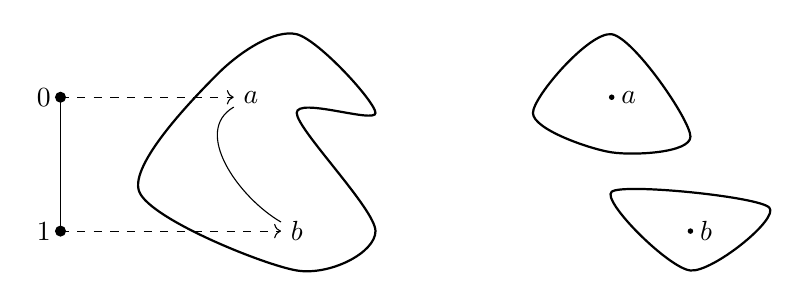
\begin{tikzpicture}
   \begin{scope}
   \draw[thick] plot[smooth cycle] coordinates{(0,0) (1,1.5) (2,2)(3, 1)(2,1)(3,-.5)(2,-1)};
   \node[right] (b) at (1.8, -.5) {$b$};
   \node[right] (a) at (1.2, 1.2) {$a$};
   \draw (a) to [out=210,in=150] (b);

   \fill(-1,-.5) circle [radius=2pt];
   \fill(-1,1.2) circle [radius=2pt];
   \draw(-1,-.5)--(-1,1.2);
   \node[left] (1) at (-1,-.5) {1};
   \node[left] (0) at (-1,1.2) {0};

   \draw[->, dashed] (0) to (a);
   \draw[->, dashed] (1) to (b);    
   \end{scope}
   \begin{scope}[xshift=5cm]
   \draw[thick] plot[smooth cycle] coordinates{(0,1) (1,2) (2,.7)(1, .5)};
   \draw[thick] plot[smooth cycle] coordinates{(1,0) (3,-.2) (2,-1)};    
   \fill(1,1.2) circle [radius=1pt];
   \fill(2,-.5) circle [radius=1pt];
   \node[right] at (1,1.2) {$a$};
   \node[right] at (2,-.5) {$b$};
   \end{scope}
  \end{tikzpicture}
 \end{center}
\end{figure}

\begin{example}
我々は事例2.1で,性質を位相空間としてモデル化した.
しかし開集合は合併で閉じているので,例えば「赤」と「緑」という性質を認めるとすると,「赤もしくは緑」という色性質も認めなければならないことになる.
これは,我々が個別に名付ける「色」は連続的に似通ったものでなければならない,という直観に反するかもしれない.
これを防ぐためには,例えば色相環のような位相空間を考え,色の性質をそのうちの弧状連結な部分集合として定義すればよい.
 \begin{center}
 \begin{tikzpicture}
 \ColourTransitionCircle[inner=1.5, outer=1.6]{yellow,red,blue,green}
 \end{tikzpicture}
 \end{center}
ここから,概念を位相的な性質によって定めるというアイデアが得られる.例えば\cite{Mormann1993-fd, Gardenfors2004-vz}などを参照.
\end{example}

% 問題:弧状連結性が同値類を形成すること

\section{同相写像}
2つの位相空間$X, Y$は,両者が集合として異なれば別物である.
しかしそれでも,例えば半径の異なる複数の円のように,位相構造としては同一視したい場合がある.
こうした同一視を可能にするのが,\emph{同相写像}(homeomorphism)である.


\begin{dfn}{同相写像}{isomorphism}
  $(X, \mcalO_X), (Y, \mcalO_Y)$をそれぞれ位相空間としたとき,$f:X \to Y$が可逆であり,$f$もその逆写像$f^{-1}:Y \to X$も連続であるとき,$f$は同相写像であるという.
  またそのとき$X$と$Y$は\emph{同相}(homeomorphic)であるという.
\end{dfn}

つまり同相写像とは両方向に連続な全単射写像である.
両方向に連続ということは,$f$で$X$の開集合を$Y$に飛ばしても$f^{-1}$で$Y$の開集合は$X$に飛ばしても,それらの像がちゃんと開集合になっている,ということである.

たとえ$X, Y$が集合として異なっていても,両者の間に同相写像があるとき,両者は位相空間としては同じものだと理解される.
というのも,位相構造を定めるのは開集合族であるが,同相写像は2つの集合の間でこれが正確に一致している,ということを保証するからだ.
したがって,同相写像があれば,2つの位相空間は実質的には同じものとして同一視して良い.
逆に,集合としては同等だが位相空間としては異なるものもある.
2章で我々は,2つの集合間に全単射写像があるとき,それらは同等である(同じ濃度を持つ)と定義した.
同等性は集合の「集合としての」同じさを定義する.
この意味では,例えば実直線$\bbR$と実平面$\bbR^2$の間には一対一の対応があるので,集合としては同等である.
しかし$\bbR^2$から$\bbR$への連続写像は存在しないので,両者の間には同相写像がなく,よって両者は「位相空間としては」同じではない.
このように,2つの数学的構造の同じさを考える際には,どのような構造としての同じさが考えられているのかに注意を向ける必要がある.
そして位相構造の場合,同一性は同相として理解されることになる.


\begin{develop}
2つの位相空間はどんなときに同相になるか,というのは位相幾何学の中心的な関心である.
一般の空間中の図形では,同相性は図形にあいた「穴の数」によって決まることが知られている.
つまり,元となる図形を,穴を開けたり塞いだりしないように連続的に変化させてもう一つの図形に変形することができたら,両者は同相である.
ここから,トポロジストにとってドーナツとマグカップは同じようなものだ,などと言われたりもする.
\end{develop}


\section{分離性}
我々は4節「さまざまな位相」で,密着位相と離散位相を両極として,細かさの異なる複数の位相があることを学んだ.
開集合を集合上の点のグルーピングとすると,位相の細かさは,個々の点をどれだけ細かく分けることができるか,ということに関係している.
実際,位相空間上の任意の異なる2点をとったとき,それらを区分する開集合があるかどうか,ということは位相空間の重要な性質であり,そうした条件は\emph{分離公理}と呼ばれている.
分離公理には複数あり,それぞれが位相空間の性質を定めているが,ここではそのうち2つを取り上げよう.

\begin{dfn}{分離公理}
位相空間$(X, \mcalO)$において,次の条件を考える:
\begin{description}
 \item[($T_0$)] 任意の異なる点$x, y$に対し,どちらかのみを含む開集合($x \in O, y \not\in O$あるいは$y \in O, x \not\in O$)が存在する.
 \item[($T_1$)] 任意の異なる点$x, y$に対し,片方ずつのみを含む開集合($x \in O_x, y \not\in O_x$および$y \in O_y, x \not\in O_y$)が存在する.
 \item[($T_2$)] 任意の異なる点$x, y$に対し,片方ずつのみを含み互いに素であるような開集合($O_x \cap O_y = \emptyset$)が存在する.
\end{description} 
特に位相空間が$(T_1)$を満たすとき\emph{フレシェ(Frechet)空間},$(T_2)$を満たすとき\emph{ハウスドルフ(Hausdorff)空間}と呼ばれる.
\end{dfn}

任意の開集合$O$は集合$X$上の「似た者」グループを表す,というイメージに沿ってそれぞれを解釈すると,
$(T_0)$では全ての点のペアについて,一方のみを含み他方を含まないという意味で両者を区分するグルーピングが存在する,ということをいっている.
フレシェ性$(T_1)$はさらに進んで,全ての点が別々にグルーピングできるということをいっている($T_0$では必ずしも両方が何らかのグループに入れられている必要性はない).
一方ハウスドルフ性$(T_2)$はそれよりもさらに強く,任意の点のペアについて,被らない仕方でグルーピング可能である,ということを要請する.

\begin{example}(Mormann 2020)
ライプニッツの\emph{不可識別者同一の原理}(the principle of the identity of indiscernibles; PII)によれば,2つのモノが全く同じ性質をもつとき,両者は同一である.つまり
\[
 \forall x, y \forall F ((Fx  \Leftrightarrow Fy) \Rightarrow x=y)
\]
ただしここで$F$は任意の一項述語を表す.
事例2.2に倣って開集合を性質の外延と考えると,これは性質の空間が$T_0$だという主張だと解釈できる.
というのも,PIIの対偶を取れば,$x\neq y$ならある性質$O_F$があって,$x \in O_F$と$y \in O_F$が同値になることがない,つまり$x \in O_F \wedge y \not\in O_F$であるか$y \in O_F \wedge x \not\in O_F$であるかのどちらかということになるが,これはまさに$(T_0)$の要件と同じだからだ.
つまりPIIとは,性質空間の位相構造についての主張だと解釈できるのである.
\end{example}

\begin{exercise}
同様に$(T_1), (T_2)$も,性質空間の特徴と考えられた場合,それぞれ何らかの同一性原理を主張していると解釈できる.
それらの間には$(T_2) \Rightarrow (T_1) \Rightarrow (T_0)$という含意関係があるので,対応する同一性原理にも強弱の違いがあるはずだ(例えば$(T_1)$に対応する同一性原理では,PIIよりも多くのものが同一とみなされうる).
それぞれの同一性基準がどのようなものか,考えてみよ.
\end{exercise}

\begin{exercise}
離散空間では,PIIはトリビアルに成立することを示せ(ヒント:離散空間で各点を区別する開集合としてどのようなものがありえるだろうか).
\end{exercise}

\begin{develop}
ここではあまり触れなかったが,これらの分離性のうちハウスドルフ性は特に色々な場面で重要である.
例えば本講では扱わないが,物理学における時空間のモデルとなる多様体(manifold)では,空間がハウスドルフ性を満たすことが要請される.
\end{develop}

%\section{距離空間}





\bibliographystyle{apalike}
\bibliography{m4p}


\end{document}